\documentclass{article}

\usepackage{generalsnips}
\usepackage{calculussnips}
\usepackage[margin = 1in]{geometry}
\usepackage{pdfpages}
\usepackage[spanish]{babel}
\usepackage{amsmath}
\usepackage{amsthm}
\usepackage[utf8]{inputenc}
\usepackage{titlesec}
\usepackage{xpatch}
\usepackage{fancyhdr}
\usepackage{tikz}
\usepackage{hyperref}
\usepackage{float}
\title{Summary Cap 1 y 2 Admin financiera}
\date{2020 August 01, 09:41PM}
\author{David Corzo}
\renewcommand{\termdefinition}[2]{
    \textbf{Definition of ``#1'':} \emph{#2}
}
\begin{document}
\maketitle
%%%%%%%%%%%%%%%%%%%%%%%%%%%%%%%%%%%%%%%%%%%%%%%%%%%%%%%%%%%%%%%%%%%%%%%%%%%%%%%%%%%%%%%%%%%%%%%%%%%%%%%%%%%%%%%%%%%%%%%%%%%%%%%%%%%%%%%%%%%%%%

{
    \LARGE\noindent \textbf{Chapter 1: An Overview of managerial Finance}
}
\section{A managerial perspective}
\begin{itemize}
    \item Rational investors hope and expect to gain wealth. 
    \item There was a problem with executives not ``acting on the best interest of investors'' this was problematic, they were paid a lot and represented huge costs to investors and in addition firing them was not a viable option because compensation plans were composed of large sums of money. 
    \item Compensation plans that limit severance payments when contracts are terminated prematurely has been recently sought, the so-called golden parachute is no longer. \termdefinition{Golden parachute}{ a package that provides executives with excessive payments when they are dismissed from their firms.} 
    \item More companies are now limiting the severance payment due. 
    \item Boards are redefining what it means to be fired for a ``just cause'', among these are poor performance and non-actions.
\end{itemize}

\section{What is finance?}
\begin{itemize}
    \item Finance is concerned with decisions about money, or more appropriately, cash flows. They deal with how money is raised by businesses, governments, and individuals. 
    \item Rational financial decisions, everything else equal:
        \begin{enumerate}
            \item More value is preferred to less. 
            \item The sooner the cash is received, the ore valuable it is. 
            \item Less risky assets are more valuable and preferred to risky assets. 
        \end{enumerate}
\end{itemize}


\section{General areas of finance}
Four interrelated areas:
\begin{enumerate}
    \item Financial markets and institutions. 
    \item Investments. 
    \item Financial services.
    \item Managerial finance. 
\end{enumerate}
\subsection{Financial markets and institutions}
\begin{itemize}
    \item Financial institutions: banks, insurance companies, savings and loans, and credit unions.
\end{itemize}
\subsection{Investments}
\begin{itemize}
    \item Focus: decisions made by businesses and individuals as they hose securities and investment portfolios.
    \item Major functions in investment: (1) determining the values, risks and returns associated with financial assets (2), determining the optimal mix of securities that should be held in a portfolio.
\end{itemize}
\subsection{Financial services}
\begin{itemize}
    \item Financial services refers to functions provided by organizations that operate in the finance industry.
    \item Banks, insurance companies, brokerage firms, and other similar companies.
    \item Provide services that help individuals(and companies) determine how to invest money. 
\end{itemize}
\subsection{Managerial (business) finance}
\begin{itemize}
    \item Managerial finance deals with decisions that all firms make concerning their cash flows.
\end{itemize}


\section{The importance of finance in non-finance areas}
\subsection{Management}
\begin{itemize}
    \item Managers concern themselves with personnel decisions and employee relations.
    \item Such personnel decisions as setting salaries, hiring new staff, and paying bonuses must be coordinated with financial decisions to ensure that any needed funds are available.
\end{itemize}
\subsection{Marketing}
\begin{itemize}
    \item Allocation of funds to do the four p's in marketing (product, price, place, and promotion).
    \item People in marketing must understand how marketing decisions affect and are affected by such issues as funds availability, inventory levels, and excess plant capacity.
\end{itemize}
\subsection{Accounting}
\begin{itemize}
    \item Financial managers rely heavily on accounting information.
    \item Accountants must understand how financial managers use accounting information in planning and decision-making so that it can be provided in an accurate and timely fashion.
    \item Accountants must understand how accounting data are viewed (used) by investors, creditors, and other outsiders. 
\end{itemize}
\subsection{Information systems}
\begin{itemize}
    \item Information system specialists work with financial managers to determine what information is needed, how it should be stored, how it should be delivered, and how information management will affect the profitability of the firm.
\end{itemize}
\subsection{Economics}
\begin{itemize}
    \item It is important that financial managers understand economics and that economists understand finance—economic activity and policy impact financial decisions, and vice versa.
\end{itemize}

\section{Finance in the organizational structure of the firm}
\begin{figure}[H]
    \centering
    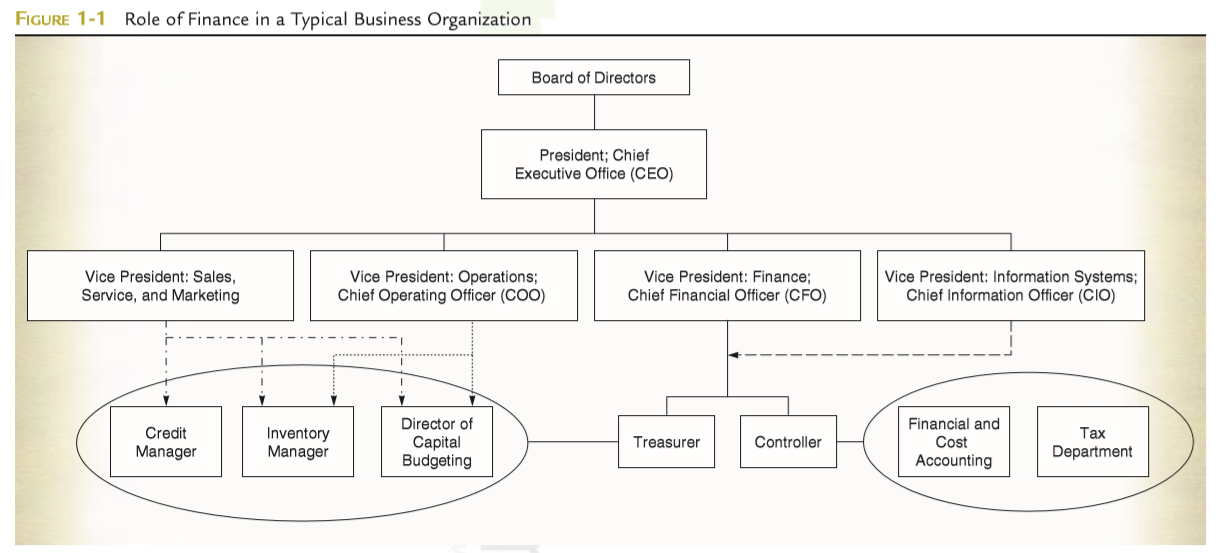
\includegraphics[width=\textwidth]{structure} 
\end{figure}


\section{Alternative forms of business organization}
3 main forms: 
\begin{enumerate}
    \item Proprietorships.
    \item Partnerships.
    \item Corporations.
\end{enumerate}
\subsection{Proprietorship 72\%-\$4\%}
\begin{itemize}
    \item \termdefinition{Proprietorship}{ is an unincorporated business owned by one individual. }
    \item 3 advantages: 
        \begin{enumerate}
            \item Easy and inexpensive to form.
            \item Fewer government regulations. 
            \item Taxed like an individual (once). 
        \end{enumerate}
    
    \item 4 Limitations:
        \begin{itemize}
            \item Unlimited personal liability for business debts. Losses can far exceed the money invested. 
            \item Limited lifetime. New owner means a new proprietorship even if the same name is used. 
            \item Transferring ownership is difficult. 
            \item Difficult to obtain large sums of capital. 
        \end{itemize}
\end{itemize}
\subsection{Partnership 8\%-\$11\%}
\begin{itemize}
    \item \termdefinition{Partnership}{ An unincorporated business owned by two or more people.} 
    \item Formality is relative: ranging from informal, oral understandings to formal agreements filed with the secretary of the state in which the partnership does business.
    \item Advantages and disadvantages of a partnership are the same as a proprietorship.
    \item 3 advantages:
        \begin{enumerate}
            \item Easy and inexpensive to form.
            \item Fewer government regulations. 
            \item Taxed like an individual (once). 
        \end{enumerate}
    
    \item 4 Disadvantages:
        \begin{enumerate}
            \item Unlimited personal liability for business debts. Losses can far exceed the money invested. 
            \item Limited lifetime. New owner means a new proprietorship even if the same name is used. 
            \item Transferring ownership is difficult. 
            \item Difficult to obtain large sums of capital. 
        \end{enumerate}
    
    \item If any partner is unable to meet his or her pro rata claim in the event the partnership goes bankrupt, the remaining partners must make good on the unsatisfied claims, drawing on their personal assets if necessary.
\end{itemize}
\subsection{Corporations 20\%-\$85\%}
\begin{itemize}
    \item \termdefinition{Corporation}{ A legal entity created by a state, separate and distinct from its owners and managers, having unlimited life, easy transferability of ownership, and limited liability. }
    \item 4 advantages:
        \begin{enumerate}
            \item Unlimited lifetime, after original owners. 
            \item Transferred more easily. Ownership interest divided into shares of stock. 
            \item Limited liability. Limited to the amount invested. 
            \item 3 previous advantages make it easy to obtain large sums of capital. 
        \end{enumerate}
    
    \item 2 disadvantages:
        \begin{enumerate}
            \item Setting up a corporation is difficult. Corporate charter (registration with the secretary of the state of the corporation) and bylaws (rules of the company).
            \item Corporate earnings are subject to double taxation.
        \end{enumerate}
\end{itemize}

\section{Hybrid business forms: LLP, LLC, S Corporation}
\begin{itemize}
    \item \termdefinition{Limited Liability Proprietorships (LLP)}{ A partnership wherein one (or more) partner is designated the general partner(s) with unlimited personal financial liability and the other partners are limited partners whose liability is limited to amounts they invest in the firm.} 
    \item \termdefinition{Limited Liability Company (LLC) }{Offers the limited personal liability associated with a corporation, but the company’s income is taxed like a partnership. } 
    \item \termdefinition{S Corporation }{A domestic corporation with no more than 75 stockholders that elects to be taxed the same as proprietorships and partnerships so that business income is taxed only once.} Advantages: 
        \begin{enumerate}
            \item Limited liability attracts investors. 
            \item Can attract funds more easily. 
            \item Ownership is easily transferable. 
        \end{enumerate}
\end{itemize}


\section{What goals should businesses pursue?}
\begin{itemize}
    \item A proprietor runs the bussiness directly and is involved in decisions made day by day. 
    \item A stockholder does not have a say and is not directly involved in the day-to-day decisions, these decisions are made by managers. Thus managers have to have the objective of \textbf{stockholder wealth maximization} and \textbf{stock price maximization}.
    \item \emph{The same actions that maximize stock prices also benefit society.}
\end{itemize}


\section{Managerial actions to maximize shareholder wealth}
\begin{itemize}
    \item The financial manager makes decisions about the expected cash flows of the firm, among these decisions are \textbf{capital structure decisions}, \textbf{capital budgeting decisions}, \textbf{dividend policy decisions}.
        \begin{itemize}
            \item \termdefinition{Capital structure decisions about how much and what types of debt and equity should be used to finance the firm. }
            \item \termdefinition{Capital budgeting decisions}{ decisions as to what types of assets should be purchased to help generate future cash flows.} 
            \item \termdefinition{Dividend policy decisions}{ decisions concerning how much of current earnings to pay out as dividends rather than retain for reinvestment in the firm.}
        \end{itemize}

    \item Although managerial actions affect the value of a firm’s stock, external factors also influence stock prices, such as: 
        \begin{itemize}
            \item Legal constraints, the general level of economic activity, tax laws, and conditions in the financial markets.
        \end{itemize}
    
    \item \termdefinition{Value }{ The present, or current, value of the cash flows an asset is expected to generate in the future.} 
\end{itemize}
\begin{figure}[H]
    \centering
    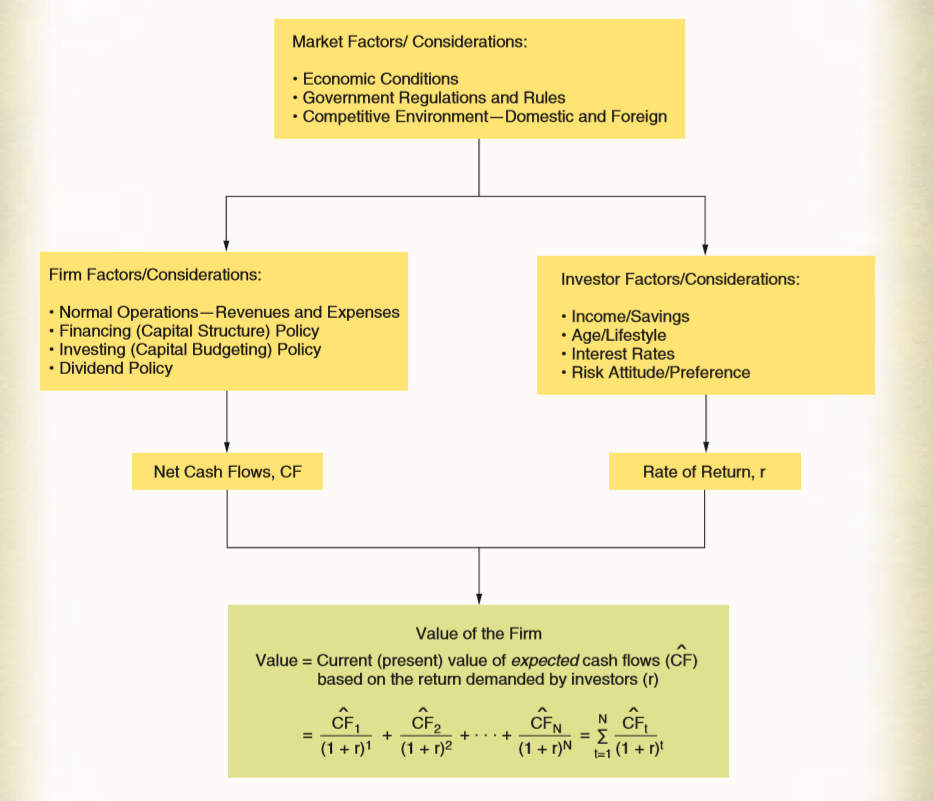
\includegraphics[width=\textwidth]{value} 
\end{figure}



\section{Should earnings per share (EPS) be maximized?}
\begin{itemize}
    \item Earnings Per Shares (EPS):  EPS receives so much attention is the belief that net income, and thus EPS, can be used as a barometer for measuring the firm’s potential for generating future cash flows.
        \[
          \text{ EPS } = \frac{\text{ Net income }}{\text{ Shares }}
        \]
    
    \item Although current earnings and cash flows are generally highly correlated, as we mentioned earlier, a firm’s value is determined by the cash flows it is expected to generate in the future as well as the risk associated with these expected cash flows. 
    \item Maximize earnings might not maximize value because earnings maximization is a short-sighted goal.
    \item Firm’s stock price, and thus its value, is dependent on, everything else equal:
        \begin{enumerate}
            \item The cash flows the firm is expected to provide in the future 
            \item When these cash flows are expected to occur 
            \item The risk associated with these cash flows. 
        \end{enumerate} 
\end{itemize}


\section{Manager's roles as agents of stockholders}
\begin{itemize}
    \item \termdefinition{Agency problem}{ A potential conflict of interest between outside shareholders (owners) and managers who make decisions about how to operate the firm.} 
        \begin{itemize}
            \item \termdefinition{Agency relationship}{  when one or more individuals, who are called the principals, hire another person, the agent to perform a service and delegate decision-making authority to that agent.} 
        \end{itemize}

    \item Mechanisms to ensure managements don't fall in agency problems: 
        \begin{enumerate}
            \item Managerial compensation (incentives): provide compensation based on a target in sales or other metric. Accomplish 2 things:
                \begin{enumerate}
                    \item Motivate management to act in the best interest of stockholders and maximize stock price. 
                    \item Attract and retain top-level executives. 
                \end{enumerate}
            
            \item Shareholder intervention: shareholders intervene and drive out management teams they consider are doing poor performance. 
            \item Threat of takeover, Hostile takeovers: The acquisition of a company over the opposition of its management.
        \end{enumerate}
    
    \item Management must pursue to maximize the price of the firm’s stock in the long term.
\end{itemize}


\section{Business ethics}
\begin{itemize}
    \item \termdefinition{Business ethics}{ A company’s attitude and conduct toward its stakeholders— employees, customers, stockholders, and so forth; ethical behavior requires fair and honest treatment of all parties.}
    \item Executives believe that there is a positive correlation between ethics and long-run profitability because ethical behavior:
        \begin{enumerate}
            \item Prevents fines and legal expenses, 
            \item Builds public trust, 
            \item Attracts business from customers who appreciate and support ethical policies, 
            \item Attracts and keeps employees of the highest caliber, and 
            \item Supports the economic viability of the communities where these firms operate. 
        \end{enumerate}
\end{itemize}


\section{Corporate governance}
\begin{itemize}
    \item The ``set of rules'' that a firm follows when conducting business; these rules identify who is accountable for major financial decisions.
\end{itemize}


\section{Forms of businesses in other countries}
\begin{itemize}
    \item Non-US firms tend to be more closed than US firms.
    \item \termdefinition{Industrial group}{ Organizations composed of companies in different industries with common ownership interests, which include firms necessary to manufacture and sell products—a network of manufacturers, suppliers, marketing organizations, distributors, retailers, and creditors.} 
\end{itemize}


\section{Multinational corporations}
\begin{itemize}
    \item \termdefinition{Multinational corporation}{ a firm that operates in two or more countries.} 
\end{itemize}
Corporation go international because they: 
\begin{enumerate}
    \item Seek new markets. 
    \item Seek raw materials.
    \item Seek new technology. 
    \item Seek production efficiency.
    \item Avoid political and regulatory hurdles. 
\end{enumerate}


\section{Multinational versus domestic managerial finance}
In theory there is no difference except for the following: 
\begin{itemize}
    \item Different currency denominations and exchange rates. 
    \item Economic and legal ramifications. 
    \item Language differences. 
    \item Cultural differences.
    \item Role of government. 
    \item Political risk (expropriation, terrorism, etc). 
\end{itemize}

{
    \LARGE\noindent \textbf{Chapter 2: Analysis of Financial Statements}
}

\section{A managerial perspective}
In the USA firms have to disclose ``fully and fairly'' all their operations, they do this by publishing financial statements and reports (these are required by the SEC \emph{Securities Exchange Commision}, FASB \emph{Finantial Accounting Standards Board}, AICPA \emph{American Intitute of Certified Public Accountants}) such as the \textbf{annual report}. \par 
Annual reports are used to communicate the financial position of the firm.
\begin{itemize}
    \item Analysis of financial statements provide information on strengths and weaknesses the firm possesses.
\end{itemize}
\subsection{Chapter 1 premises}
\begin{itemize}
    \item Stock's value is determined by the cash flows that the firm is expected to generate in the future. 
    \item Managers must strive to maximize the value of the firm's stock. 
    \item To estimate value, both managers and investors must be able to estimate future cash flows.
\end{itemize}

\section{Recording business activity — financial statements}
\begin{itemize}
    \item Birth of accounting was 4,000 years ago. 
    \item The need to record transactions became prevalent as a way of proof and a way to settle disputes. 
    \item 15th century modern accounting was born with Benetto Cotrugli (double entry bookkeeping system).
    \item Luca Pacioli formally developed the double entry system.
    \item Financial books have historically provided important information about the financial well-being of businesses.
\end{itemize}


\section{Financial reports}
\begin{itemize}
    \item \termdefinition{Annual report}{ This report describes the firm's operating results during the past year and discusses new developments that will affect future operations and gives an accounting picture of the firm's operations and financial position.} 
        \begin{itemize}
            \item It includes a verbal section, presented as a letter of the chairman describing what happened and what is in store for the future. 
            \item It includes:  
                \begin{enumerate}
                    \item The balance sheet. 
                    \item The income statement. 
                    \item Statement of cash flows. 
                    \item Statement of retained earnings. 
                \end{enumerate}
        \end{itemize}
    
    \item Investors use the information contained in the annual report to form expectations about future earnings and dividends.
\end{itemize}


\section{Financial statements}
\subsection{The balance sheet}
\begin{itemize}
    \item \termdefinition{Balance sheet }{ This financial statement represents a picture taken at a specific point in time (date) that shows a firm's assets and how those assets are finances (debt or equity)}.
        \begin{figure}[H]
            \centering
            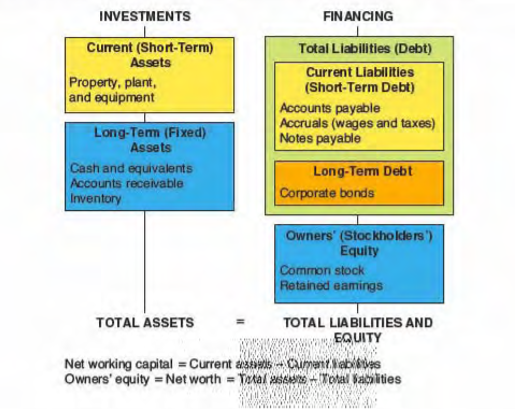
\includegraphics[]{\figs/balance} 
        \end{figure}

    \item \termdefinition{Common stockholders' equity or net worth }{ The total assets minus total liabilities. } 
        \begin{itemize}
            \item Net worth implies, but does not mean, that the stockholders get distributed the net worth in its entirety. 
        \end{itemize}
    
    \item \termdefinition{Retained earnings }{ An account that effectively represents the total amount of income a company has saved and reinvested in assets since it started business. It shows the cumulative amount of income the company has kept rather than paid out as dividends over the years. } 
        \begin{itemize}
            \item If bad debts are written off int the assets section of the balance sheet, the retained earnings balance is reduced in the equity section. 
        \end{itemize}
    
    \item Common equity is composed of common stock and retained earnings. 
     
    \item Ways of listing items in a balance sheet: Started by Pacioli in 15th century.
        \begin{itemize}
            \item Assets are listed in the order of their ``liquidity''.
            \item Claims (liabilities and equity) listed in order of which must be paid. 
        \end{itemize}
    
    \item \termdefinition{Common size balance sheet}{ Items on a balance sheet that are stated as percentages. Used to compare with other firms.} 
\end{itemize}

Additional points:
\begin{enumerate}
    \item Cash and equivalents versus other assets: assets $\neq$ cash, except in the case of cash and equivalents.
    \item Accounting alternatives: firms can use LIFO or FIFO for inventories, and different depreciation methods such as accelerated and straight line, sometimes for fiscal reasons. 
    \item Breakdown of the common equity account: in some firms the equity account is composed by commons stock and retained earnings, in other firms common equity sections can be composed of common stock at par, paid-in capital, and retained earnings. 
        \[
          \text{ Common stocks at par }= \text{ Total shares issued }\times \text{ share par value }
        \]
    
    \item Book values versus market values: book values of assets often do not equal their market values (depreciation), book values of debts are usually very close, the difference between them results in equity. Differences between the book value and market value of equity primarily depends on the differences between the book values and market values of the firm's assets. 
        \begin{itemize}
            \item \termdefinition{Book values}{ the values or accounting numbers, that are reported on the balance sheet and are generated using generally accepted accounting principles (GAAP).} 
            \item \termdefinition{Market values}{ the prices (values) for which assets can actually be sold in the marketplace. } 
        \end{itemize}
    
    \item The time dimension: A firms balance sheet will change throughout the year depending on the date on which the statements are constructed.
\end{enumerate}

\subsection{Income statement}
\begin{itemize}
    \item \termdefinition{Income statement}{ Also referred to as profit and loss statement. It presents the results of business operations during a specified period of time such as a quarter or a year and summarizes the revenues generated and the expenses incurred bu the firm during the accounting period.} 
    \item The EPS (Earnings Per Share) are presented at the bottom. 
\end{itemize}

\subsubsection{Should identical firms report the same net income?}
\begin{itemize}
    \item No, they might be financed differently, one with debt and the other with equity. 
\end{itemize}

\subsubsection{Does net income determine value?}
\begin{itemize}
    \item 
\end{itemize}


%%%%%%%%%%%%%%%%%%%%%%%%%%%%%%%%%%%%%%%%%%%%%%%%%%%%%%%%%%%%%%%%%%%%%%%%%%%%%%%%%%%%%%%%%%%%%%%%%%%%%%%%%%%%%%%%%%%%%%%%%%%%%%%%%%%%%%%%%%%%%%
\end{document}

